%!TEX root = ../main-anran-ma.tex 
% so I can build in this tex file too. 
%************************************************
% \setcounter{theorem}{6}
\chapter{Necessary Liberal Preconditions}\label{ch:nlp} % $\mathbb{ZNR}$
%************************************************

% \section{Literature Review}

% Here is a description of all the triples. 
% \todo{Literature review section}



We are interested in studying the \define{necessary liberal precondition}, a weakening of the weakest liberal precondition: 
$$wlp.C.F\implies G$$
We show our interest, by relating all the pre- and postcondition transformers, so we can distinguish the existing triples that are already well-researched graphically. 

Luckily, we can find scenarios where the overapproximation can be useful, and demonstrate it with an example, before giving a proof system. 
We conclude that this overapproximation can help us find more preconditions that can lead to failure, either by including states that lead to unidentified errors, or by including states that can lead to errors via non-terministic choice. 
The latter method then leads to finding conditions that are able to capture these special states. 
The side effect of this result is that we can now find the wlp transformer with angelic non-determinism using wlp with demonic non-determinism and sp.

This chapter includes our most important results: 
\begin{enumerate}
	\item The predicate transformers are all related together nicely by relations like termination, reachability, conjunction, over- and under-approximation, and implication in both directions. 
	\item Without any additional constraints, the necessary liberal preconditions can be anything. The only thing we are sure of is that its negation guarantees termination in the negation of the desired postcondition. 
	\item Necessary liberal preconditions find their usefulness in avoiding bugs. 
	\item With necessary liberal precondition, we also can overapproximate and underapproximate wlp with angelic non-determinism ($wlp_a$). In the end, we can qualify $wlp_a$ using necessary liberal precondition and strongest postcondition transformers, without having to define $wlp_a$.  
\end{enumerate}


In the upcoming sections, we first relate together wp, wlp, sp, and slp with both angelic and demonic non-determinism, so we can distinguish the necessary liberal precondition from the existing triples that are already well-studied. 
In this chapter, we first discuss the general semantics of the necessary liberal precondition, then focus on a characteristic scenario and show properties that captures it. 

\section{Relating Overapproximations of wlp and sp}\label{sec:negative}
Recall that in \autoref{sec:literature}, we mentioned that there is an equivalence relation between the underapproximation of wlp and the overapproximation of sp via a Galois connection: 
\begin{align}
	G\implies wlp.C.F\text{\ \ \ \ iff\ \ \ \   } sp.C.G\implies F \tag{*}
\end{align}
One might wonder whether we can also establish some similar relation between the overapproximation of wlp and the underapproximation of sp:  
\begin{align}
	wlp.C.F \implies G\ \ \ \  \rlap{\(\quad?\)}\longleftrightarrow \ \ \ \ F\implies sp.C.G \tag{**}
\end{align}
This would imply that we merely need to study the underapproximation of $sp$ to result in the overapproximation of $wlp$, where the underapproximation of $sp$ is studied as the (total) incorrectness triple~\cite{ohearn2020IncorrectnessLogic}. 

The answer is no. 
Without additional constraints, we can not directly establish any implication relations between $wlp.C.F\implies G$ and $F\implies sp.C.G$. 

Remember from \autoref{ch:appr} that all initial states that guarantee non-termination satisfy $wlp.C.F$, and that $sp.C.G$ is satisfied only by final states that are reachable. 
Termination and reachability are two different aspects of program execution. 
If we denote explicitly the states that can lead to non-termination with blue squares, and states that are unreachable with orange circles, then we can see on the left half of \autoref{fig:wlp-sp-nonterm-reach} that $F$ can also be satisfied by unreachable states, and from the right half that $G$ can also be satisfied by states leading to non-termination.
In general, without further constraints, $F$ in \autoref{fig:wlp-sp-nonterm-reach} is decorated with \imptt{some} of the orange circles, and $G$ is decorated with \imptt{some} of the blue squares. 

\begin{figure}[ht]
	\centering
	\includesvg[width=\linewidth]{image/wlp-sp-nonterm-reach.svg}
	\caption{Non-Terminating and Unreachable States}
	\label{fig:wlp-sp-nonterm-reach}
\end{figure}

As an example, consider the program 
$$C=if\ (x=2)\ then\ \{x:=x+2\}\ else\ \{x:=x+1\}$$
and a postcondition $F=\{x>2\}$.
We can deduce the weakest liberal precondition: 
\begin{align*}
	wlp.C.F &= \{x=2\}\wedge (wlp.x:=x+2).F\ \vee\ \{x\neq 2\} \wedge wlp.(x:=x+1).F\\
	&\Leftrightarrow\{x=2\}\wedge \{x>0\}\  \vee \ \{x\neq 2\}\wedge\{x>1\}\\
	&\Leftrightarrow\{x=2\} \vee \{x>2\}\\ 
	&\Leftrightarrow \{x\geq 2\}
\end{align*}
As a result, as long as the program $C$ starts in an initial state satisfying $x\geq 2$, it will terminate in a state satisfying $F=\{x>2\}$. 
However, a state where $x$ evaluates to $3$ would satisfy $F$, but it is never reachable: assume the else-branch was executed, then $x$ must evaluate to $2$ initially, but else-branch will only be executed when $x\neq 2$ and this assumption leads to contradiction; otherwise assume the if-branch was executed, then $x$ must initially evaluate to $1$, but then the if-branch would not be executed. 
Hence, any state where $x$ evaluates to $3$ is unreachable, but still satisfies the desired postcondition $F$. 
Such states are denoted as orange circles in \autoref{fig:wlp-sp-nonterm-reach}. 
Similarly, $sp.C.F$ can also be satisfied by initial states that can lead to non-termination.

Attempting to establish a relation for line (**), we first start from the left side. 
Assume preconditions $G$ satisfies $wlp.C.F\implies G$, we can end up in a situation like \autoref{fig:wlp-g-sp-g}. 

\begin{figure}[ht]
	\centering
	\includesvg[width=\linewidth]{image/wlp-g-sp-g.svg}
	\caption{$sp.C.G$ where $G$ Is Overapproximation of $wlp.C.F$}
	\label{fig:wlp-g-sp-g}
\end{figure}

\newcommand{\nimplies}{\rlap{\(\quad\not\)}\implies} %symbol for not implies
We see on the left side of \autoref{fig:wlp-g-sp-g} that $G$ ``includes'' all the blue squares, and $F$ only some of the orange circles. 
Now what do we know about $sp.C.G$? 
We see on the right side of \autoref{fig:wlp-g-sp-g}, $sp.C.G$ is only satisfied by reachable states, i.e. none of the orange circles. 
This means that in general, without further constraints, we can not always conclude that $F\implies sp.C.G$, since $F$ may be satisfied by unreachable states, but $sp.C.G$ is only satisfied by reachable states. 

Can we then always have a relation like $sp.C.G\implies F$ for arbitrary $G$ and $F$? 
The answer is no. Assume we have both $wlp.C.F\implies G$, and $sp.C.G\implies F$, then with the Galois connection mentioned in line (*), we can conclude that $G\implies wlp.C.F$, which means that $G\Leftrightarrow wlp.C.F$, $G$ must be \imptt{exactly} the weakest liberal precondition of $F$. 
Since we can only assume that $G$ overapproximates wlp, we can not draw the conclusion that $sp.C.G\implies F$. 
As a result, from $wlp.C.F\implies G$ we can neither conclude $sp.C.G\implies F$ nor $F\implies sp.C.G$. 

Analogously, assume $F\implies sp.C.G$, what can we state about $wlp.C.F$?
\begin{figure}[ht]
	\centering
	\includesvg[width=\linewidth]{image/f-sp-wlp-f.svg}
	\caption{$wlp.C.F$ where $F$ Is Underapproximation of $sp.C.G$}
	\label{fig:f-sp-wlp-f}
\end{figure}
From the left side of \autoref{fig:f-sp-wlp-f}, we can see that $F$ does not ``include'' orange circles, i.e. $F$ is only satisfied by reachable states. 
What do we know then about the relation between $wlp.C.F$ and $G$? 
We see from \autoref{fig:f-sp-wlp-f}, $wlp.C.F$ ``includes'' all the blue squares, but $G$ only some of them. 
Consequently, we can not conclude that $wlp.C.F\implies G$. 
Also, we can not conclude that $G\implies wlp.C.F$, because this would require $sp.C.G\implies F$. 
Together with the assumption $F\implies sp.C.G$, this means that $F$ must be \imptt{exactly} the strongest postcondition of program $C$ w.r.t. precondition $G$, also a luxury we can not assume. 

Summarizing the two conclusions above together, we can say that in general, without further constraints: 
\begin{itemize}
	\item From $wlp.C.F\implies G$, we can neither conclude $F\implies sp.C.G$ nor $sp.C.G\implies F$;
	\item Analogously, from $F\implies sp.C.G$ we can neither conclude $wlp.C.F\implies G$ nor $G\implies wlp.C.F$. 
\end{itemize}
This tells us that we can \imptt{not} overapproximate wlp by underapproximating sp, at least not directly. 



% However, only having information about $F\implies sp.C.G$ like the right side of \autoref{fig:wlp-sp-nonterm-reach} tells us nothing about the distribution of blue squares: in general, $G$ might only ``include'' part of the blue squares. 
% Hence, we can not establish a relation 

% At the same time, let $G=\{x\geq 2\}$ then 
% \begin{align*}
% 	&sp.C.G \\
% 	&= sp.(x:=x+2).(\{x=2\}\wedge\{x\geq 2\})\ \vee\ sp.(x:=x+1).(\{x\neq 2\}\wedge\{x\geq 2\})\\
% 	&= sp.(x:=x+2).\{x=2\}\ \vee\ sp.(x:=x+1).\{x> 2\}\\
% 	&= \exists a.x=(x+2)[x/a]\wedge \{x=2\}[x/a]\  \vee \ \exists a.x=(x+1)[x/a]\wedge \{x>2\}[x/a]\\
% 	&\Leftrightarrow \exists a.x=a+2\wedge \{a=2\}\  \vee \ \exists a.x=a+1\wedge \{a>2\}\\
% 	&\Leftrightarrow\{x=4\} \vee \{x>3\}\\
% 	&\Leftrightarrow \{x\geq 4\}
% \end{align*}

% In other words, $sp.C.G$ is only satisfied by reachable final states, not by any final state where $x$ evaluates to $3$. 
% Consequently, any postcondition $F'$ such that $F'\implies sp.C.G$ must not be satisfied by any state $\tau$ where $\tau.x=3$. 
% But all such states $\tau$ automatically satisfy $F=\{x>2\}$ , but any state $G'$ where $wlp.C.F\implies G'$ must be satisfied by all states where 




\section{The General Case}\label{sec:general}
As hinted before, in our triple $wlp.C.F\implies G$, $G$ overapproximates wlp. 
It can take different forms: on the one hand, $G$ can be so general that it is satisfied by any program state; on the other hand, a $G$ that is barely weaker than $wlp.C.F$ is also not much different from the latter. 
Alternatively, $G$ can also be all kinds of preconditions that starting from it, any postcondition is reachable. 
One thing we are certain about, though, is that a program with an original state satisfying $\neg G$ will terminate, and the final state can satisfy $\neg F$: 
\begin{align*}
wlp.C.F{\implies} G & \Leftrightarrow \neg G {\implies} \neg wlp.C.F \\
	& \Leftrightarrow \neg G {\implies} wp.C.\neg F 
	\hspace{0.2\textwidth} \mid {\thm{conjugate}}
\end{align*}
These equivalences indicate that \hoare{\neg G}C{\neg F} is a valid Hoare triple with respect to total correctness, i.e. if $C$ starts in an initial condition satisfying $ \neg G$, then its execution \imptt{must} terminate, and it must be able to terminate satisfying $\neg F$. 

% \subsection{Overapproximation of wlp}
In \autoref{sec:wlp} we define the weakest liberal precondition and state that it characterizes all the preconditions starting from which the program either \imptt{diverges} or \imptt{will} terminate in a state satisfying $F$. 
We are certain to use ``will'' instead of ``can'' as the non-deterministic choice is viewed as demonic, so the behavior of wlp can be depicted by \autoref{subfig:wlpd}. 

The rectangle on the left (right) denote the set of all initial (final) states $\S$. 
$C$ is the program, and its executions are depicted by arrows. 
The rectangle is divided into halves, the part with label $wlp.C.F$ denotes all the states that satisfy $wlp.C.F$, and so on. 
The dashed arrow starting from inside a rectangle, ending outside neither rectangle denotes executions that do not terminate. 
The arrows that share the same point from the left rectangle denote different executions starting from the same initial state. 

Starting from one initial state, the execution of the program can take various forms: it can be strictly deterministic, or it can have multiple non-deterministic choices; it can terminate in a final state, or it can execute forever. 
We categorize the executions of the program in four ways: 
\begin{enumerate}
	\item the dashed arrow means non-terminating executions; 
	\item the black arrows are executions starting from an initial state satisfying $wlp.C.F$ and if they terminate, then only terminating in final states satisfying $F$; 
	\item the green arrows are the executions starting from an initial state satisfying $\neg wlp.C.F$ but are always possible to terminate in states either satisfying $F$ or satisfying $\neg F$;
	\item the red arrow represents executions starting from an initial state satisfying $\neg wlp.C.F$ and only terminating in final states satisfying $\neg F$. 
\end{enumerate}


\begin{figure}[ht]\centering
	\subfloat[Weakest liberal precondition (demonic non-determinism)\label{subfig:wlp-g}]{
		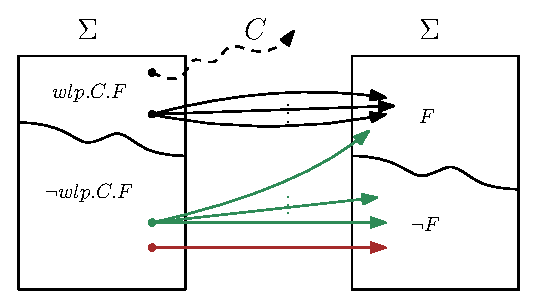
\includegraphics[width=0.4\textwidth]{image/wlp-g/wlpd.eps}}
	\hfill

	\subfloat[Precondition $G$ with $wlp.C.F\implies G$ and $G$ contains some green arrows\label{subfig:wlp-g-g}]{
		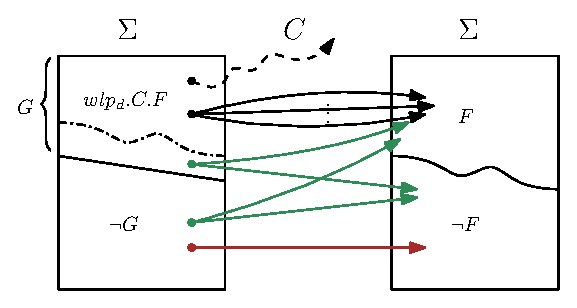
\includegraphics[width=0.45\textwidth]{image/wlp-g/wlp-g-g.eps}
	}
	\hfill
	\subfloat[Precondition $G$ with $wlp.C.F\implies G$ and $G$ contains all the green arrows\label{subfig:wlp-g-gg}]{
		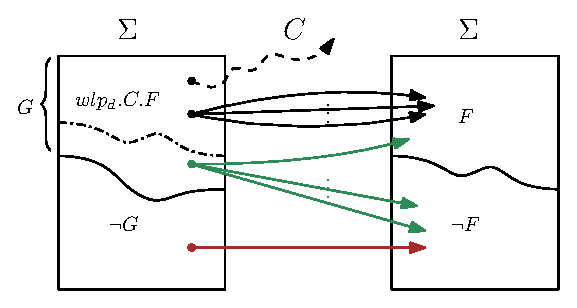
\includegraphics[width=0.45\textwidth]{image/wlp-g/wlp-g-gg.eps}
	}

	\subfloat[Precondition $G$ with $wlp.C.F\implies G$ and $G$ contains some red arrows\label{subfig:wlp-g-r}]{
		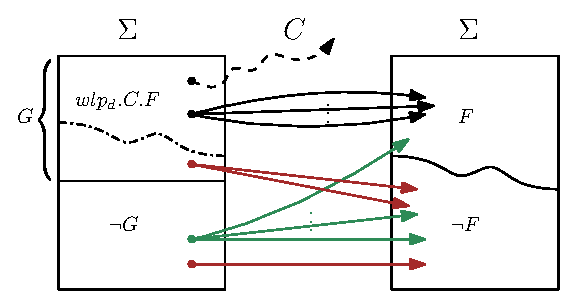
\includegraphics[width=0.45\textwidth]{image/wlp-g/wlp-g-r.eps}
	}
	\hfill
	\subfloat[Precondition $G$ with $wlp.C.F\implies G$ and $G$ contains all the red arrows\label{subfig:wlp-g-rr}]{
		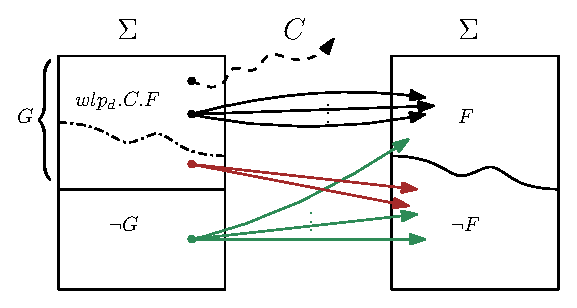
\includegraphics[width=0.45\textwidth]{image/wlp-g/wlp-g-rr.eps}
	}
\caption{Case Distinction of Preconditions Weaker Than wlp}
\label{fig:wlp-g-1}
\end{figure}

\begin{figure}[ht]\centering
	\ContinuedFloat
	\subfloat[Precondition $G$ with $wlp.C.F\implies G$ and $G$ contains some green arrows and some red arrows\label{subfig:wlp-g-gr}]{
		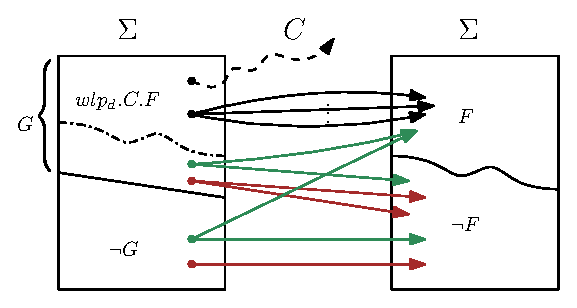
\includegraphics[width=0.45\textwidth]{image/wlp-g/wlp-g-gr.eps}
	}
	\hfill
	\subfloat[Precondition $G$ with $wlp.C.F\implies G$ and $G$ contains all the green arrows and some red arrows\label{subfig:wlp-g-ggr}]{
		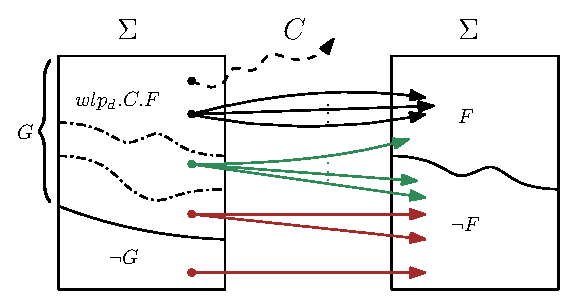
\includegraphics[width=0.45\textwidth]{image/wlp-g/wlp-g-ggr.eps}
	}

	\subfloat[Precondition $G$ with $wlp.C.F\implies G$ and $G$ contains some green arrows and all the red arrows\label{subfig:wlp-g-grr}]{
		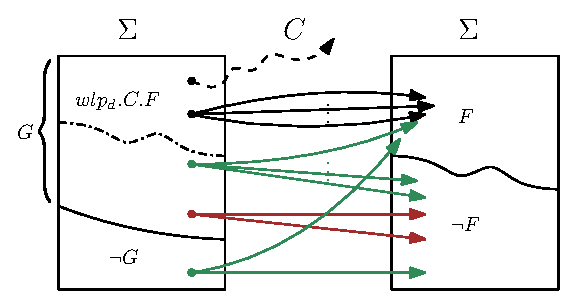
\includegraphics[width=0.45\textwidth]{image/wlp-g/wlp-g-grr.eps}
	}
	\hfill
	\subfloat[Precondition $G$ with $wlp.C.F\implies G$ and $G$ contains all the arrows\label{subfig:wlp-g-ggrr}]{
		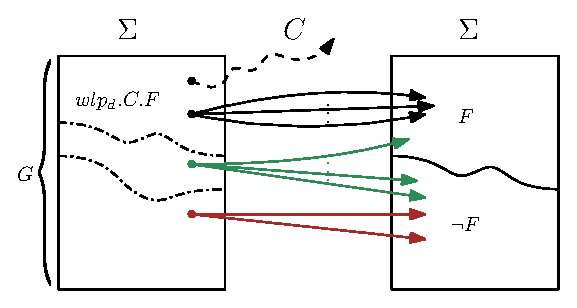
\includegraphics[width=0.45\textwidth]{image/wlp-g/wlp-g-ggrr.eps}
	}
\caption{Case Distinction of Preconditions Weaker Than wlp (Cont.) }
\label{fig:wlp-g-2}
\end{figure}

Without additional constraints, if we were to weaken the precondition, a lot of cases exist, and we can not make many statements about the weakened precondition. 
Various scenarios are shown in \autoref{subfig:wlp-g}{\color{RoyalBlue}-9}. 
For example, \autoref{subfig:wlp-g} shows the situation where $G$ is exactly $wlp.C.F$. 
But in \autoref{subfig:wlp-g-g}, $G$ is strictly weaker than $wlp.C.F$. 
Here, $G$ is satisfied by all initial states that satisfy $wlp.C.F$, plus \imptt{some} of the initial states, starting from which the execution can end satisfying $F$ or $\neg F$, aka some of the green arrows. 
Further, the $G$ in \autoref{subfig:wlp-g-gg} is satisfied by \imptt{all} the above initial states, i.e. all the green arrows start from $G$. 
The same principle applies to the red arrows. 
\autoref{subfig:wlp-g-r} shows a $G$ that is satisfied additionally by \imptt{some} of the initial states that are starting points of the red arrows, i.e. executions that start in $\neg wlp.C.F$, and end in $\neg F$. 
In \autoref{subfig:wlp-g-rr}, $G$ contains all such initial states. 

The situation can be trickier, for example in \autoref{subfig:wlp-g-gr}, $G$ is also the starting point of both green and red arrows. 
In other words, if $C$ starts from some initial state satisfying this $G$, then maybe its execution diverges, maybe it terminates satisfying $F$, maybe not. 
The same can be said about the $G$ in \autoref{subfig:wlp-g-ggr} and \autoref{subfig:wlp-g-grr}. 
Finally, $G$ is weakened so much that it is simply $true$, hence satisfied by all initial states as seen in \autoref{subfig:wlp-g-ggrr}. 
We see that there are a lot of possibilities on how to overapproximate wlp. 
Furthermore, the analysis shown in \autoref{fig:wlp-g-1} is not accounting for the gray arrows depicted in \autoref{subfig:wlpd-extended}, the addition of which would make the number of cases explode even more. 

% We thus first investigate this special case, before proceeding with $G$ in general. 

% While having restrictions on $G$ yields interesting results, without the restrictions we can still find useful characteristics. 
In general, when $wlp.C.F\implies G$, $G$ can be satisfied by all possible initial states, which can be the starting points of black, green, red, or dashed arrows, representing executions terminating in states satisfying $F$, $F$ or $\neg F$, $\neg F$, or non-terminating, respectively. 
As a result, we can not make many statements about the states in $G$ without adding extra restrictions to $G$. 

However, we can see from \autoref{subfig:wlpd}{\color{RoyalBlue}-9} that when $\neg G$ is not empty, there is always some arrow ending in $\neg F$. 
So there always exists some execution that starts from an initial state satisfying $\neg G$, and ends in a final state satisfying $\neg F$%: \hoare{\neg G}C{\neg F} is a valid hoare triple. 

Alternatively, we can say that does not contain any \imptt{black} or \imptt{dashed} arrows in all cases. 
In other words, if program $C$ starts in any initial state satisfying $\neg G$, then either $G$ is empty, or
\begin{itemize}
	\item its executions terminate, and
	\item there exists an execution that ends up in a final state that satisfies $\neg F$. 
\end{itemize}

This again states that \hoare{\neg G}{C}{\neg F} is a valid Hoare triple. 
The question then naturally arises: why do we concern ourselves with $G$, if we can just prove our specifications using wp or Hoare triples? 
To demonstrate the answer, we analyze the example in the upcoming sections. 


% \subsection{Example: Door with Sensors}
\subsection{Example: To Exclude Bugs}
The necessary liberal precondition can also be regarded as a method to rule out bugs. 
In the author's student life, there was a door at university that she always finds interesting. 
The door is located at a lecture hall, equipped with two sensors on the left and right sides of the door frame. 
Each time a person walks in or out, the sensor registers and adds or decreases the number of people in the lecture hall, making a small tick sound. 
It seems that this door serves the purpose of helping security guards keep an eye on the lecture rooms after closing time without having to be physically there. 

But can the door really distinguish from a person entering or leaving the room? 
And what if naughty students try to trick the door by using a backpack to pretend to exit the door multiple times? 
What if one of the sensors break? 
We can this simple scenario by putting the three parts in non-deterministic choice. 
It can happen that a student enters the room hence increasing the count of the number of people present: $n:=n+1$; or a person exits and decreasing the number: $n:=n-1$. 
Alternatively, the sensor can break because of old age and result in unforeseeable behavior, for example always detecting someone entering forever. 
The pseudocode is shown in \autoref{lst:door}. 

\begin{lstlisting}[caption={Door with Sensors Counting Number of People Present}, label={lst:door}, language=java, numbers=left, stepnumber=1, captionpos=b,escapechar=|,frame=single]
	... // starting device
	n := n + 1 |$\square$| n := n - 1 |$\square$| diverge;|\label{line:tri-nondet}|
	... // retirement  
\end{lstlisting}

We know that there is definitely something wrong, in case the security sees on their device that the number of people in a lecture hall is negative. 
One way to try to exclude bugs is to find it the precondition, upon whose violation the program is prone to erroneous termination. 
With this view, we name the bugs that we are aware of, like $P$ in \autoref{fig:bug}. 
Then we calculate the weakest precondition of $P$ with regard to program $C$, then take its negation. 
Consequently, its negation $Q$, the purple area in \autoref{fig:bug}, is an overapproximation of $wlp.C.F$, where $F$ is the postcondition that the program execution is bug free. 

Specifically, if we were to violate the necessary liberal precondition $Q$, the execution of program $C$ is prone to terminate in erroneous states that we know of, namely that there are a negative number of people in the room. %, or that there are over $200$ people in the room. 
However, starting in an initial state satisfying $Q$ does not guarantee that the executions are completely bug-free. 
Since we may not have complete knowledge of all the error states, we can still encounter executions starting form $Q$ ending in an error state, in this case the red arrow in \autoref{fig:bug} that points to the error state ``people present during holidays'' or ``capacity of lecture hall $200$ exceeded''. 
In conclusion, the use of necessary liberal precondition can help us avoid bugs that we have knowledge over. 

\begin{figure}[t]
	\centering
	\includesvg[width=\linewidth]{image/bugs.svg}
	\caption{Necessary Liberal Precondition to Avoid Bugs}
	\label{fig:bug}
\end{figure}

This is one way to approach bug-avoidance: by the negation of the weakest precondition. 
Another way is to try to overapproximate wlp directly. 

If we want to know what caused it, we can calculate the weakest liberal precondition of the program snippet with regard to $F=\{\sigma\in\S\mid\sigma.n<0\}$, the result in \autoref{lst:neg0}. 
We write $F=\{n<0\}$ in short: 
\begin{lstlisting}[caption={Weakest (Liberal) Precondition w.r.t Postcondition $F=\{\sigma\in\S\mid\sigma.n<0\}$ }, label={lst:neg0}, language=java, numbers=left, stepnumber=1, captionpos=b,escapechar=|,frame=single]
	... // starting device
	|\imptt{$\{n<-1\}$}|
	|\imptt{$\{n<-1\}\ \wedge\ \{n<1\}\ \wedge\ true$}|
	n := n + 1 |$\square$| n := n - 1 |$\square$| diverge;
	|\imptt{\{$n<0$\}}|
	... // retirement   
\end{lstlisting}

It seems like we should avoid starting the system in a state where $n$ is less than $-1$. 
But it is enough? If we start the system in a state where $n=-1$, or even $n=0$, we can still reach an erroneous state where the value of $n$ is negative. 
% \autoref{fig:door}
\begin{figure}[ht]
	\centering
	\includesvg[width=0.7\linewidth]{image/example-door.svg}
	\caption{$wlp.C.F = \{n<-1\}$}
	\label{fig:door}
\end{figure}
We can see that with wlp, it is not enough to identify all preconditions that can result in errors. 
In other words, the green arrows in \autoref{fig:door} are not recognized. 
This tells us that wlp is so strict that it excludes the green arrows, and the reason could be that the resolution of non-termination is demonic. 
However, by overapproximating wlp to include preconditions like $\{n=-1\}$ and $\{n=-1\}$, we can also include all the green arrows in $G$. 

On the other hand, as earlier, we might only have limited knowledge of all potential bugs in the system. 
The lecture hall does not have unlimited capacity. 
Once the system is showing a number higher than the maximum capacity, we know that an error happened. 
Also, there could be conditions like ``during holiday time, the lecture halls are unoccupied'' that an expert of the system (the security guards in this case) would know, but not in general. 
By overapproximatin wlp even more, we might end up in a situation like in \autoref{fig:door-expert}, where the red arrows are also ``included'' in $G$.

\begin{figure}[ht]
	\centering
	\includesvg[width=0.8\linewidth]{image/example-door-expert.svg}
	\caption{$wlp.C.F \implies G$}
	\label{fig:door-expert}
\end{figure}

These two aspects of the example demonstrate the usefulness of the overapproximation of wlp: We can find a precondition, the violation of which would definitely lead to erroneous final states, and we can find a precondition, whose avoidance is necessary to avoid executions leading to bugs. 




\subsection{Example: Including Good Runs}
Another reason one might wish to overapproximate the weakest liberal precondition is that wlp might be so strict that some good runs are excluded. 
Cousot et al. discovered patterns in System.dll that demonstrates this effect~\cite{cousot13}. 
\begin{lstlisting}[caption={Good Runs Excluded}, label={lst:run}, language=java, numbers=left, stepnumber=1, captionpos=b,escapechar=|,frame=single]
	... 
	for (int i = 0; i <= a.length; i++){
		a[i] = ...f(a[i])...; 
		if (NonDet()) return; 
	}
	...
\end{lstlisting}
In this example in \autoref{lst:run}, $a[i]$ is an array, the function $NonDet()$ is a non-deterministic function that returns boolean values. 
At run time, an out-of-bound error may or may not appear at line 3, depending on what happened before and after $f(a[i])$, the value of $i$ may or may not be modified, or the array $a$ may or may not be changed. 
To achieve out-of-bound-error-free, the weakest (liberal) precondition of this program snippet would be $false$: 
If the $NonDet()$ function in line 4 returns $false$ for some times, there is  \imptt{no} guarantee that error will not appear at line 3. 

We can see from \autoref{fig:run} that $wlp.C.F$ empty, and it rules out some good runs like the green ones. 
However, $G=a.length>0$ is an overapproximation over wlp, and it includes some good runs as indicated by the green arrows. 
These green arrows indicate runs where $Nondet()$ returns $false$ for some times, so the program continues to run, but returning $false$ and ending the program execution before an out-of-bound could happen. 
From the same initial state, we can be unlucky and $NonDet()$ returns $false$ for some more times, so that line 3 is executed for a couple of times more, and out-of-bound error happened, indicated by the red arrows in \autoref{fig:run}.

\begin{figure}[ht]
	\centering
	\includesvg[width=.85\linewidth]{image/run.svg}
	\caption{Overapproximating wlp to Include Good Runs}
	\label{fig:run} 
\end{figure}

This example tells us that the weakest (liberal) precondition might be too strict at times, and it rules out good runs of program execution. 
By overapproximating wlp, we end up with a more relaxed precondition, starting from which even though bad runs are still possible, we still capture some good executions that would otherwise be excluded. 




\subsection{Proof System}\label{sec:system}
\newcommand{\nlp}[3]{\langle #1 \rangle\ #2\ \langle #3 \rangle}
We call the overapproximation of wlp \define{necessary liberal precondition}, ``necessary'' because it is required to ensure avoidance of erroneous final states, and ``liberal'', because it is satisfied by all initial states that can potentially lead to non-termination, just like wlp. 
We provide a proof system in \autoref{tab:proof-system}. 
We use $\nlp G C F$ to denote that $G$ is a valid necessary liberal precondition for program $C$ given postcondition $F$. 

The rules are mostly unsurprising. 
Remember that we would like to construct rules to prove that a precondition is the necessary liberal precondition, it should overapproximate the weakest liberal precondition, i.e. a triple $\nlp G C F$ should satisfy: 
$$wlp.C.F \implies G$$
Consequently, we have the $diverge$ axiom: because $wlp.diverge.F=true$, and $true$ is the only condition that overapproximates it, so the necessary liberal precondition is $true$.  

Consequently, we have the $skip$ axiom: because $wlp.skip.F = F$, then $F$ overapproximates it. 
Alternatively, we can construct the rule in such way: 
\begin{center}
	\begin{prooftree}
		\Hypo{F{\implies} G}
		\infer1[$skip_{alt}$]{\nlp {G} {skip} { F}}
	\end{prooftree}
\end{center}
But this rule can be derived using the $skip$ rule and the $conseq$ in \autoref{tab:proof-system}, so we choose the simpler $skip$ rule. 
The same principle applies to the $assign$, $seq$, $if$, and the $choice$ rule: we keep the rules simple by not discussing overapproximation directly, but let the $conseq$ rule be concerned with relaxation. 

The consequence rule says that we are allowed to weaken the precondition and strengthen the postcondition: 
$$\displaystyle\frac{P{\implies} G,\ \nlp P C Q,\ F{\implies} Q}{\nlp{G}{C}{F}} conseq$$
Intuitively, if a precondition $P$ already overapproximates the weakest liberal precondition, then by overapproximating it with $G$, the result is still an overapproximation of wlp: 
$$wlp.C.F\implies P \implies G$$
Conversely, we can strengthen the postcondition from $Q$ to $F$, because $wlp.C$ is monotonic (\autoref{thm:wlp-mono}), then given $ F\implies Q $ we can derive: 
$$wlp.C.F\implies wlp.C.Q\implies G$$ 
Hence, $G$ is still an overapproximation of the stronger $wlp.C.F$. 

Note that the $conseq$ rule is the complete opposite direction from the ``Rules of Consequence'' in Hoare logic that we referred to in \autoref{tab:hoare}. 
Writing the consequence rule of Hoare logic in the same natural deduction style, we arrive at the following rule labeled with $conseq_h$: 
$$\displaystyle\frac{G{\implies} P,\ \hoarenm{P}{C}{Q},\ Q{\implies} F}{\hoarenm{G}{C}{F}}conseq_h$$
This corresponds to our expectation, because we know that the overapproximation triple is exactly a Hoare triple (with respect to partial correctness) with negated pre- and postconditions:
\begin{align*}
	& \ wlp.C.F{\implies} G \\
	\Leftrightarrow &\  \neg G {\implies} \neg wlp.C.F \\
	\Leftrightarrow &\  \neg G \implies wp.C.\neg F 
		\hspace{0.3\textwidth} \mid {\thm{conjugate}} \\
	\Leftrightarrow &\  \hoarenm{\neg G}C{\neg F} 
	\tag{*} 
\end{align*}
Note that the last line is an implication in both directions, because we take the version of Hoare triple regarding total correctness, i.e. supplementing the rule to prove termination of while loops~\cite{manna74}: 
\begin{center}
	\begin{prooftree}
		\Hypo{$\hoare{P\wedge\varphi\wedge v\in\N\wedge v=n\ \ }{C}{\ \ P\wedge v\in\N\wedge v<n}$}
		\infer1[$while_h$]{$\hoare {P\wedge v\in\N\ \ } {while\ (\varphi)\ do\ C} {\ \ \neg\varphi\wedge P\wedge v\in\N}$}
	\end{prooftree}
\end{center}
% In other words, \hoare{\neg G}C{\neg F} can be a valid Hoare triple with respect to partial correctness, but an initial state satisfying $\neg G$ does not necessarily guarantee termination, hence $\neg G$ is not necessarily a subset of $wp.C.\neg F$. 
% If we were to take Hoare triple with additional rules to prove termination~\cite{manna74}, the implication at line (*) would be in both directions. 
We also give intuition of the consequence rule in our proof system.
Assuming that the triple $\nlp\cdot\cdot\cdot$ is sound (which we will prove later in this section), i.e. $\nlp P C Q \implies (wlp.C.F{\implies} G)$, we can derive the $conseq$ rule from $consqe_h$  : 
\begin{center}
	\begin{prooftree}
		\Hypo{P{\implies} G,\ \nlp P C Q,\ F{\implies} Q}
		\infer1[soundness]{P{\implies} G,\ wlp.C.Q{\implies} P,\ F{\implies} Q}
		\infer1[(*)]{P{\implies} G,\ \hoarenm{\neg P}C{\neg Q},\ F{\implies} Q}
		\infer1[first-order logic]{\neg G{\implies} \neg P,\ \hoarenm {\neg P} C {\neg Q},\ \neg Q{\implies} \neg F}
		\infer1[$conseq_h$]{\hoarenm {\neg G} C {\neg F}}
		\infer1[(*)]{wlp.C.F\implies G}
		\infer1[(soundness)]{\nlp{G}{C}{F}}
	\end{prooftree}
\end{center}

\begin{table}[t]
  \normalsize
  \centering
  \framebox{
  $\begin{array}{@{}ccc@{}}
  \displaystyle\frac{}{\nlp F {skip} F} skip &
  \displaystyle\frac{}{\nlp {true} {diverge} F} div 
  \\[3ex]
  \displaystyle\frac{}{\nlp {F[x/e]} {x:=e} F} assign &
  \displaystyle\frac{\nlp G {C_1} P,\ \nlp P {C_2} F}{\nlp G {C_1; C_2} F} seq &
  \\[3ex]
  \displaystyle\frac{\nlp {\varphi\wedge G} {C_1} F,\ \nlp {\neg\varphi\wedge G} {C_2} F}{\nlp{G}{IF}{F}} if &
%   \displaystyle\frac{\nlp {\varphi\wedge F\wedge v=n} {C'} {F\vee v>n},\ v,n\in\N}{\nlp {\varphi\vee F} {WHILE} {F}} while &
%   \displaystyle\frac{\nlp {\varphi\wedge v=n} {C'} {v>n},\ v,n\in\N}{\nlp {\varphi\vee F} {WHILE} {F}} while &
% \displaystyle\frac{\forall P\in\P.\ \nlp {\varphi\wedge P} {C'} {\varphi}}{\nlp {\varphi\vee F} {WHILE} {F}} while &
%   \displaystyle\frac{P\implies\neg\varphi}{\nlp {P\wedge F} {WHILE} {F}} while_0 &
%   \displaystyle\frac{\nlp {P} {C} {\varphi\vee P}}{\nlp {P} {WHILE} {\varphi\vee P}} while &
\displaystyle\frac{\forall X=\Phi(X):\nlp {P} {C} {X}}{\nlp {P} {WHILE} {\varphi\vee P}} while
%   \displaystyle\frac{\nlp {P} {C} {F}}{\nlp {P\vee F} {WHILE} {F}} while_2 &
  \\[3ex]
  \displaystyle\frac{\nlp G {C_1} F,\ \nlp G {C_2} F}{\nlp G {C_1\square C_2} F} choice &
  \displaystyle\frac{P{\implies} G,\ \nlp P C Q,\ F{\implies} Q}{\nlp{G}{C}{F}} conseq 
  \\[3ex]
  \text{ where } IF= if\ (\varphi)\ \{C_1\}\ else\ \{C_2\}\text{, }
  & WHILE= while\ (\varphi)\ do\ \{C\}, 
  \\
  \Phi(X):=\neg\varphi\wedge P \ \vee\  \varphi\wedge wlp.C.X
\end{array}$}
  \caption{The Proof System}
  \label{tab:proof-system}
\end{table}

It is however not trivial to construct the while rule. 
Assume we would like to find some $G$ to overapproximate $wlp.WHILE.F$, unfolding according to the definition in \autoref{tab:wp-wlp}: 
\begin{align*}
	wlp.WHILE.F &= gfp\ X. \Phi(X)\\  
	&= gfp\ X.\ (\neg\varphi\wedge F)\vee(\varphi\wedge wlp.C.X) 
\end{align*}
Since $G$ overapproximates $wlp.WHILE.F$, the greatest fixed point of $\Phi$, then $G$ must also overapproximate any fixed point of $\Phi$: 
For any fixed point $P$ of $\Phi$, it must be valid that $P\implies gfp\ \Phi$. 
Together with $gfp\ \Phi\implies G$, we can conclude that $P\implies G$. 
In other words, the weakest liberal precondition $G$ must overapproximate all fixed points of $\Phi$: 
\renewcommand{\iff}{\Leftrightarrow}
\begin{align*}
	&\forall P. P=\Phi(P): P\overset{!}{\implies} G\\  
	\iff \ &\forall P=\Phi(P). (\neg\varphi\wedge F)\vee(\varphi\wedge wlp.C.P)\overset{!}{\implies} G\\  
	\iff \ &\forall P=\Phi(P). (\neg\varphi\wedge F) \overset{!}{\implies} G 
	\ \ \wedge\ \ 
	(\varphi\wedge wlp.C.P)\overset{!}{\implies} G\\  
\end{align*}
The first conjunct can be fulfilled by choosing $G=(\neg\varphi\wedge F)\ \vee\cdots$, however, the overapproximation of the second conjunct is not straightforward. 
Remember from \autoref{sec:define loops} that when $P$ is a fixed point of the characteristic function $\Phi$ and $P$ is not the least fixed point, then $P$ is satisfied by initial states starting from which non-termination is possible. 
Now that we need to overapproximate all $wlp.C.P$ where $P$ is a fixed point of the characteristic function, we need to ``capture'' all initial states where non-termination is possible. 
In other terms, we need to prove non-termination. 
One approach would be to first prove termination, then take the negation. 

Again, we try to get intuition from the while-rule in Hoare logic, namely the $while_h$ above. 
Since we are doing informal deduction, we replace $v\in\N$ with $v\geq 0$ to give nicer formulas when negated.
This helps us rewrite the $while_h$ rule into $while_h'$: 
\begin{center}
	\begin{prooftree}
		\Hypo{$\hoare{P\wedge\varphi\wedge v\geq 0\wedge v=n\ \ }{C}{\ \ P\wedge v\geq 0\wedge v<n}$}
		\infer1[$while_h'$]{$\hoare {P\wedge v\geq 0\ \ } {while\ (\varphi)\ do\ C} {\ \ \neg\varphi\wedge P\wedge v\geq 0}$}
	\end{prooftree}
\end{center}
% Assume that the upper line of $while_h'$ is proven, then
% \begin{align*}
% 	&\nlp {\neg(P\wedge\varphi\wedge v\geq 0\wedge v=n)} {C} {\neg(P\wedge v\geq 0\wedge v<n)} \tag{**}
% \end{align*}
% should also be valid. 
% Line (**) is equivalent to: 
% \begin{align*}
% 	&(**)\\
% 	\iff & \nlp {\neg P\vee\neg \varphi\vee v< 0\vee v\neq n} {C} {\neg P\vee v<0\vee v\geq n}\\
% 	\iff & wlp.C.(\neg P\vee v<0\vee v\geq n)\implies (\neg P\vee\neg \varphi\vee v< 0\vee v\neq n)\\ 
% 	\iff & (wlp.C.\neg P\implies (\neg P\vee\neg \varphi\vee v< 0\vee v\neq n))\\ 
% 	&\ \ \wedge (wlp.C.(v<0)\implies (\neg P\vee\neg \varphi\vee v< 0\vee v\neq n))\\
% 	&\ \ \wedge (wlp.C.(v\geq n)\implies (\neg P\vee\neg \varphi\vee v< 0\vee v\neq n)) \tag{***}\\ 
% \end{align*}
% The last equivalence, noted with (***), is derived from the monotonicity of $wlp.C$ (\thm{wlp-mono}) and the fact that $A\implies A\vee B$ for all predicates $A$, $B$. 
Let $WHILE = while\ (\varphi)\ do\ C$. 
Following the principle that \hoare{G}C F is a valid Hoare triple if and only if $\nlp {\neg G} C {\neg F}$ is a valid necessary liberal precondition triple, from the bottom line of $hoare_h'$ we \imptt{should} be able to prove that 
\begin{align*}
	& \nlp {\neg(P\wedge v\geq 0)} {while\ (\varphi)\ do\ C} {\neg(\neg\varphi\wedge P\wedge v\geq 0)} \text{ should be valid}\\
	\iff\ & \nlp{\neg P\vee v< 0} {while\ (\varphi)\ do\ C} {\varphi\vee \neg P\vee v< 0} \text{ should be valid}\\
	\iff\ & wlp.WHILE.(\varphi\vee \neg P\vee v< 0)\ \  \overset{!}{\implies}\neg P\vee v< 0\\
	\iff \ & gfp\ X.\ \neg\varphi\wedge(\varphi\vee \neg P\vee v< 0) \ \ \vee\ \  \varphi\wedge wlp.C.X  \ \ \overset{!}{\implies}\neg P\vee v< 0\\
	\iff \ & gfp\ X.\ \neg\varphi\wedge (\neg P\vee v< 0) \ \ \vee\ \  \varphi\wedge wlp.C.X  \ \ \overset{!}{\implies}\neg P\vee v< 0 \tag{e}\\
\end{align*}
Finally, let $\Phi(X):=\neg\varphi\wedge (\neg P\vee v< 0) \ \vee\  \varphi\wedge wlp.C.X$, 
we can see that the necessary and sufficient condition to achieve line (e) is: 
\begin{align*}
	& \forall X=\Phi(X):\neg\varphi\wedge (\neg P\vee v< 0) \ \ \vee\ \  \varphi\wedge wlp.C.X  \ \ \implies \neg P\vee v< 0 \\ 
	\iff \ & \forall X=\Phi(X):(\neg\varphi\wedge (\neg P\vee v< 0) \ \implies \neg P\vee v< 0) \\ 
	& \hspace{.15\linewidth} \wedge\ \  (\varphi\wedge wlp.C.X \implies \neg P\vee v< 0)  \\ 
	\iff \ &\forall X=\Phi(X): \  \varphi\wedge wlp.C.X \implies \neg P\vee v< 0  \tag{h}\\ 
\end{align*}
And a sufficient condition to arrive at line (h) is that:
$$\forall X=\Phi(X):  wlp.C.X \implies \neg P\vee v< 0 $$
This condition corresponds to the validity of $\nlp{\neg P\vee v< 0}{C}{X}$, for all fixed points of $\Phi(X)$. 
This choice is enough for us to construct a sound proof system.%, but we will see that the resulted proof system is not complete. 
As a result, syntactically replacing $\neg P\vee n<0$ by $P$, we can construct a while-rule: 
$$\displaystyle\frac{\forall X=\Phi(X):\nlp {P} {C} {X}}{\nlp {P} {WHILE} {\varphi\vee P}} while$$

\begin{lemma}{sound-pf}[The proof system is sound]
	\ \\
	$$\nlp G C F\implies (wlp.C.F{\implies} G)$$
\end{lemma}

\begin{proof}
	We prove by induction and case distinction over the lowest level of the proof tree. 
	\paragraph{Cases $skip$, $div$, $assign$} Straightforward.
	\paragraph{Case $seq$} 
	Assume we proved the triple $\nlp G {C_1;C_2} F$ with the following proof tree: 
	\begin{center}
		\begin{prooftree}
			\infer0{\cdots}
			\infer1{\cdots\cdots}
			\infer1{}
			\Ellipsis{}{ }
			\infer1{\nlp G {C_1} P,\ \nlp P {C_2} F}
			\infer1[$seq$]{\nlp G {C_1;C_2} F}
		\end{prooftree}
	\end{center}
	Then we have proven $M_1:=\nlp G {C_1} P $ and $M_2:=\nlp P {C_2} F $ as the premises of the last deduction, as well as $M_3:=\nlp G {C_1;C_2} F$ as the conclusion of the last deduction step.
	We also have the induction hypotheses $$H_1:=\nlp G {C_1} P {\implies} (wlp.C_1.P{\implies} G)$$ 
	$$H_2:=\nlp P {C_2} F {\implies} (wlp.C_2.F{\implies} P)$$
	Our goal is to prove $\nlp G {C_1;C_2} F {\implies} (wlp.(C_1;C_2).F{\implies} G)$. 
	By discharging $M_1$ in $H_1$, $M_2$ in $H_2$, and $M_3$ in the goal, we acquire premises $wlp.C_1.P{\implies} G$ and $wlp.C_2.F{\implies} P$ to prove goal $wlp.(C_1;C_2).F{\implies} G$. 
	This is done by discharging of the definition of wlp with composition and the monotonicity of wlp: 
	\begin{align*}
		&\ wlp.(C_1;C_2).F = wlp.C_1.(wlp.C_2.F) 
		\hspace{0.1\linewidth}\mid \text{definition of wlp} \\
		\Rightarrow &\ wlp.C_1.P  
		\hspace{0.433\linewidth}\mid \text{monotonicity of wlp}\\
		\Rightarrow &\ G  
		\hspace{0.527\linewidth}\mid \text{premise}
	\end{align*}

	\paragraph{Case $if$}
	Unrolling the definition of $wlp.IF.F$ we get that 
	$$wlp.IF.F = \varphi\wedge wlp.C_1.F\ \vee\ \neg\varphi\wedge wlp.C_2.F$$ 
	Similar as before, by discharging induction hypotheses and premises, we can acquire the following conditions: 
	$$wlp.C_1.F\implies\varphi\wedge G \text{ and }
	 wlp.C_2.F\implies\neg\varphi\wedge G $$
	From the first condition we get: 
	$$\varphi\wedge wlp.C_1.F\implies wlp.C_1.F \implies \varphi\wedge G\implies G$$
	and 
	$$\neg\varphi\wedge wlp.C_2.F\implies wlp.C_2.F \implies \neg\varphi\wedge G\implies G$$
	Hence $wlp.IF.F \implies G$. 
	\paragraph{Case $while$}
	From the induction hypothesis we can derive that 
	\begin{align*}
		&\forall X=\Phi(X):  wlp.C.X\implies P \\
		\implies\ & \forall X=\Phi(X): \varphi\wedge wlp.C.X\implies P 
	\end{align*}
	It is a fact that $\neg\varphi\wedge P \implies P$, from $\neg\varphi\wedge P \iff \neg\varphi\wedge (\varphi\vee P)$ we can deduce that $$\neg\varphi\wedge (\varphi\vee P) \implies P$$. 
	Combining with the previous result, we get that 
	$$\forall X=\Phi(X):  \neg\varphi\wedge P  \ \ \vee \ \ \varphi \wedge wlp.C.X\implies P$$
	Because 
	$\Phi(X) = \neg\varphi\wedge P \ \vee\  \varphi\wedge wlp.C.X$, we can conclude that 
	\begin{align*}
		& gfp \ X. \  \neg\varphi\wedge P  \ \ \vee \ \ \varphi \wedge wlp.C.X\implies P\\
		\iff &\ gfp \ X. \  \neg\varphi\wedge (\varphi\vee P)  \ \ \vee \ \ \varphi \wedge wlp.C.X\implies P
	\end{align*}
	Hence, 
	$wlp.WHILE.(\varphi\vee P)\implies P$, and we have proved our goal.

	\paragraph{Case $choice$} Similar to the case with $seq$, we can prove that $$wlp.(C_1\square C_2).F \implies G$$ from 
	$$wlp.(C_1\square C_2).F = wlp.C_1.F \wedge wlp.C_2.F$$
	and 
	$$wlp.C_1.F \implies G\ \wedge\ wlp.C_2.F \implies G$$

	\paragraph{Case $conseq$}
	This case is also not different from before: from the induction hypotheses and premises we can derive $wlp.C.Q \implies P$. 
	Together with $P\implies G$, $F\implies Q$ and the monotonicity of $wlp.C$ we conclude that 
	$$wlp.C.F\implies wlp.C.Q \implies P \implies G$$
\end{proof}

% \begin{lemma}{incomplete-pf}[The proof system is incomplete]
% 	here 
% \end{lemma}

% \begin{proof}
% 	here 
% \end{proof}


\section{A Special Case}\label{sec:special} %: $G$ is wlp with Angelic Non-determinism
As promised before, we will look into a way to identify the green arrows in \autoref{fig:door}, aka the executions that start from initial states but may end non-deterministically in $F$ or $\neg F$. 
We can easily see that if we overapproximate wlp by adding all the green arrows, we end up with \autoref{subfig:wlp-g-gg}, which is exactly wlp with angelic non-determinism, as shown in \autoref{fig:wp-family} at the beginning of this chapter. 

When $G$ corresponds to \autoref{subfig:wlp-g-gg}, we know that under its control, the program always \imptt{can} reach a final state satisfying $F$ if it terminates, while with an initial state satisfying $\neg G$, the program is \imptt{will} terminate satisfying $\neg F$.
This behavior describes exactly the behavior of wlp with angelic non-determinism, which is more obvious if we put together \autoref{subfig:wlp-g-gg} and  \autoref{subfig:wlpa}: 
\begin{figure}[ht]
	\centering
	\raisebox{.2\height}{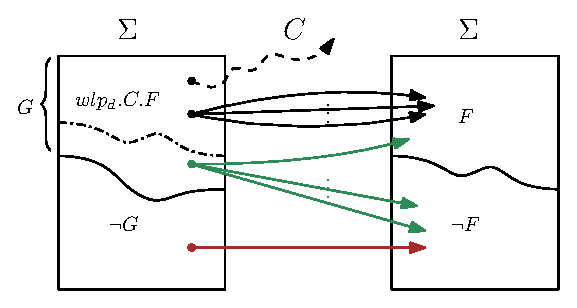
\includegraphics[width=.45\linewidth]{image/wlp-g/wlp-g-gg.eps}}
	\hfill 
	\includesvg[width=.42\linewidth]{image/wlpa.svg}
	\label{wlp-g-wlpa}
	\caption{Comparing $G$ With Angelic wlp}
\end{figure}
% However, $G$ spikes our interest when it takes the form as in \autoref{subfig:wlp-g-gg}, because under its control, the program always \imptt{can} reach a final state satisfying $F$ if it terminates, while with an initial state satisfying $\neg G$, the program is \imptt{will} terminate satisfying $\neg F$. 
% This behavior is exactly the behavior of wlp, if we were to regard the non-deterministic choice as angelic, as hinted by the similarities between \autoref{subfig:wlp-g-gg} and \autoref{subfig:wp-angelic}. 

Unfortunately, we can not use either big-step semantics in \autoref{sec:big-step} or collecting semantics in \autoref{sec:collecting} to describe the intended semantics of wlp with angelic resolution of non-determinism. 
The reason is that both semantics can not easily distinguish between executions of programs like $C_1\square diverge$ and $skip$, but angelic wlp would require the distinction. 
Fixing an initial state $\sigma$, with big-step semantics, we can only state about the program $C_1\square diverge$ that $\sigma$ can take a big step to whichever state the program $C_1$ can take it to: 
\begin{center}
	\begin{prooftree}
		\hypo{\sigma\ar{C_1}\tau}
		\infer1[$choice_1$]{\sigma\ar{C_1\square diverge}\tau}
	\end{prooftree}
\end{center}
Hence, given a transition where $\sigma C\tau$, we do not know whether a big step towards $\tau$ is the only step $\sigma$ can take with program $C$, or it is one of the steps, and another possible step leads to non-termination. 

Similarly, with collecting semantics, we have that 
$$\semb{C_1\square diverge}{\sigma} = \semb{C_1}{\sigma}\cup\semb{diverge}{\sigma}= \semb{C_1}{\sigma}\cup\emptyset= \semb{C_1}{\sigma}$$ 
Hence, the collecting semantics of $C_1\square diverge$ and $C_1$ are the same. 
For the above reasons, we attempt to capture the intended behavior of wlp with angelic non-determinism (denoted by \define{wlp$_a$}) with case distinction of different groups of executions with help of graphical illustration. 
We show the graphs of wp, wlp, wlp$_a$, and sp together in \autoref{fig:wp-wlp-wlpa-sp}. 

\begin{figure}[ht]\centering
	\subfloat[Weakest precondition (angelic non-determinism)\label{subfig:wpa-proof}]{
		\includesvg[width=0.4\textwidth]{image/wpa-extended.svg}}
	\hfill
	\subfloat[Weakest liberal precondition (demonic non-determinism)\label{subfig:wlpd-proof}]{
		\includesvg[width=0.4\textwidth]{image/wlpd-extended.svg}}
	\hfill\subfloat[Strongest postconditoin (angelic non-determinism)\label{subfig:spa-proof}]{
		\includesvg[width=0.4\textwidth]{image/spa.svg}}
	\hfill\subfloat[Weakest liberal precondition (angelic non-determinism)\label{subfig:wlpa-proof}]{
		\includesvg[width=0.4\textwidth]{image/wlpa-extended.svg}}
	\hfill
\caption{wp$_a$, wlp$_d$, sp$_a$, wlp$_a$ Together}
\label{fig:wp-wlp-wlpa-sp}
\end{figure}

To help with reasoning, given program $C$ and postcondition $F$, we consider its executions and categorize the initial states into the following disjoint sets: 
\begin{itemize}
	\item $S_{FF}$: the set of all initial states where starting from any state in this set, all executions terminate, and the final states satisfy $F$. 
	\item $S_{nFnF}$:the set of all initial states, where starting from any state in this set, all executions terminate, and the final states satisfy $\neg F$. 
	\item $S_{FnF}$: the set of all initial states, where starting from any state in this set, at least one execution diverges, at least one execution terminates and the final state satisfies $F$, and at least one execution terminates and the final state satisfies $\neg F$. 
	\item $S_{II}$: the set of all initial states, where starting from any state in this set, all executions diverge. The subscript $I$ stands for ``infinite''. 
	\item $S_{IF}$: the set of all initial states, where starting from any state in this set, at least one execution diverges, and at least one execution terminates, and the final state satisfies $F$. 
	\item $S_{InF}$: the set of all initial states, where starting from any state in this set, at least one execution diverges, and at least one execution terminates, and the final state satisfies $\neg F$. 
	\item $S_{IFnF}$: the set of all initial states, where starting from any state in this set, at least one execution diverges, at least one execution terminates and the final state satisfies $F$, and at least one execution terminates and the final state satisfies $\neg F$. 
\end{itemize}

Similarly, given program $C$ and precondition $G$, we can categorize the final states into the following disjoint sets: 
\begin{itemize}
	\item $T_{U}$: the set of all unreachable final states. 
	\item $T_{GG}$: the set of all reachable final states, where all executions leading to it originally started in an initial state satisfying $G$. 
	\item $T_{nGnG}$: the set of all reachable final states, where all executions leading to it originally started in an initial state satisfying $\neg G$. 
	\item $T_{GnG}$: the set of all reachable final states, where looking at any of them, there exists at least one execution reaching this final state originated in an initial state satisfying $G$, and there exists at least one execution reaching this final state originated in an initial state satisfying $\neg G$. 
\end{itemize}

Studying \autoref{fig:wp-wlp-wlpa-sp}, we see that the states satisfying wp with angelic resolution of non-determinism can be characterized as: 
Starting from this state, termination in a final state satisfying $F$ is always possible. 
More concretely, starting from an initial state satisfying $wp_a.C.F$, there can exist executions where it diverges, or terminates in a final state satisfying $\neg F$, but there \imptt{must} exist at least one execution where it terminates, and the final state satisfies $F$. 
As a result, We can then characterize $wp_a.C.F$ as the following: 
\[wp_a.C.F = S_{FF}\cup S_{FnF}\cup S_{IF}\cup S_{IFnF}\]

Similarly, the states satisfying $wlp_d.C.F$ can be characterized as: 
Starting from any of these states, either all executions lead to final states satisfying $F$ upon termination, or non-termination is guaranteed. 
Consequently, 
\[wlp_d.C.F = S_{FF}\cup S_{II}\cup S_{IF}\]

The states satisfying $sp_a.C.G$ can be characterized as: 
There must exist an execution from an initial state satisfying $G$ that reaches this final state. 
\[sp_a.C.G = T_{GG}\cup T_{GnG}\]

The states satisfying $wlp_a.C.F$ should behave like the following: 
Starting from any of these states, either non-termination is guaranteed, or there must be an execution with final state satisfying $F$, or some of the executions diverge, and others terminate in a final state satisfying $\neg F$. 
As a result, 
\[wlp_a.C.F = S_{FF}\cup S_{FnF}\cup S_{IF}\cup S_{InF}\cup S_{IFnF}\cup S_{II} =\S-S_{nFnF}\]


% as ``if $C$ starts in an initial state satisfying $wlp_a.C.F$, then its execution either is possible to diverge, or is possible to end in a state satisfying $F$'', 
% then we can deduce its semantics as follows, recalling the representation for non-termination mentioned in \autoref{sec:big-step}: 
% \begin{statement}{wlpa-sound}[Semantics of $wlp_a$]%TODO
% \ \vspace{-1.5mm}
% \[
% WRONG!!! wlp_a.C.F = \{ \sigma\in\S \mid
% \neg(\exists \tau\in\S: \sigma\goto{C}\tau) \ \ \vee\ \ 
% (\exists \tau\in\S: \sigma\goto{C}\tau\wedge  \tau\vDash F)
%  \}
% \]
% % \label{thm:wlpa}
% \end{statement}
We propose that we can find $wlp_a$ by using the necessary liberal precondition and the strongest postcondition. 
While trying to distinguish what is and is not in $wlp_a$, we approach it in two directions: first, we find restraints that make the necessary liberal precondition $G$ where $wlp.C.F\implies G$ an overapproximation of angelic wlp ($ wlp_a.C.F \implies G$); then we find restraints that makes $G$ an underapproximation of angelic wlp. 
Finally, we combine both directions and conclude with statements that make $G$ and $wlp_a.C.G$ equivalent. 
We also gain a side effect of expressing wlp$_a$ without having to define it. 

\begin{lemma}{wlpa-g}[Angelic wlp implies G]
\ \\ \vspace{-3mm}
	\[\hspace{-2mm}
	\text{ if \ \ \ \ } 
	(wlp_d.C.F\implies G)
	\ \wedge\ 
	(sp_a.C.\neg G \implies \neg F) 
	\text{\ \ \ \  then\ \ \ \  } 
	wlp_a.C.F \implies G
	\] 
	\label{lem:wlp-g}
\end{lemma}
The second prerequisite \mathl{sp.C.\neg G \implies \neg F } states that from $\neg G$ we are only allowed to reach $\neg F$, making sure that all green arrows as in \autoref{fig:wlp-g-1} are included in $G$. 

\renewcommand{\iff}{\Leftrightarrow}
\begin{proof}
	Rewriting the statements above, we get:
	\begin{align*} 
	wlp_d.C.F{\implies} G
	&\iff S_{FF}\cup S_{II}\cup S_{IF} \implies G \tag{a} \\
	sp_a.C.\neg G{\implies}\neg F 
	&\iff T_{nGnG}\cup T_{GnG} \implies \neg F \\ 
	&\iff F\implies \neg(T_{nGnG}\cup T_{GnG}) \\
	&\iff F\implies \S-(T_{nGnG}\cup T_{GnG}) \\
	&\iff F\implies T_{GG}\cup T_{U} \tag{d}\\
	wlp_a.C.F{\implies} G
	&\iff S_{FF}\cup S_{FnF}\cup S_{IF}\cup S_{InF}\cup S_{IFnF}\cup S_{II}  \implies G \tag{e} 
	\end{align*}
	To prove line (e), comparing line (a) and line (e) we see that we only need to prove that 
	$$S_{FnF}\cup S_{InF}\cup S_{IFnF} \implies G $$
	From line (d) we see that final states in $F$ are either unreachable from any initial state, or can only be reached via executions starting from initial states satisfying $\neg G$. 
	Since $T_U$ and ${T_nGnG}$ are disjoint, there are two separate cases. 
	The first case is that $F\implies T_{U}$, then for any state $\tau\in F$, we know that there exists no execution that has $\tau$ as final state, so all $S\_$ with ``there exists at least one execution that terminates in a final state satisfying $F$'' as part of their descriptions are empty, i.e. $S_{FnF}, S_{IF}, S_{IFnF}$. 
	Hence, in this case, we have that 
	$S_{FnF}\cup S_{InF}\cup S_{IFnF} \implies G $. 
	
	The second case is that $F\implies T_{GG}$, this means that for any state $\tau\in F$, there exists and only exists executions leading to $\tau$ that start from an initial state satisfying $G$. 
	This means that any $S\_$ with ``there exists at least one execution that terminates in a final state satisfying $F$'' must be a subset of $G$. 
	Consequently, $ S_{FnF}\cup S_{InF}\cup S_{IFnF} \implies G $ is valid in this case as well. 
\end{proof}

% macros for referencing to lines in this chapter
% \newcommand{\lblth}[1]{\hypertarget{3.#1}{{\text{#1}}}}
% \newcommand{\refth}[1]{\hyperlink{3.#1}{{\text{Line (#1)}}}}
% \begin{proof}
% 	The assumption expresses that for any state $\sigma\in\S$:
% \begin{align*} 
% 	wlp.C.F\implies G\  \Leftrightarrow&\ \sigma\in wlp.C.F \implies \sigma\in G \\
% 	\Leftrightarrow&\ ( \forall \tau\in\S:\ \sigma\goto{C}\tau\implies  \tau\in F) \implies \sigma\in G \tag*{$\mid$ \thm{wlp-sound}} \\
% 	\Leftrightarrow&\ (\forall \tau\in\S:\ \neg(\sigma\goto{C}\tau)\ \vee\ \tau\in F) \implies \sigma\in G \\
% 	\Leftrightarrow&\ \neg(\exists\tau\in\S:(\sigma\goto{C}\tau)\ \wedge\ \neg(\tau\in F)) \implies \sigma\in G \tag{\lblth{a}} \\
% 	% && \mid \lblth{a} \\
% 	% &\ \ \ \  \vee (\forall \tau.\sigma\goto{C}\tau:\tau\in F \Longrightarrow \sigma\in G) 
% 		% \hspace{0.017\textwidth} \mid \lblth{b} \\
% 	%
% \end{align*}
% Also, for any state $\tau\in\S$: 
% \begin{align*}
% 	sp.C.\neg G \implies \neg F \Leftrightarrow&\ \tau\in sp.C.\neg G \implies \tau\in \neg F \\
% 	\Leftrightarrow&\  (\exists \mu\in\S:\ \mu\goto{C}\tau\ \wedge\ \mu\in\neg G )\implies \tau\in\neg F \tag*{$\mid$ \thm{sp-sound}}\\
% 	% &\hspace{0.45\textwidth} \mid \thm{sp-sound}\\
% 	\Leftrightarrow&\  \neg (\tau\in\neg F) \implies \neg (\exists \mu\in\S:\ \mu\goto{C}\tau\ \wedge\ \mu\in\neg G ) \\
% 	\Leftrightarrow&\  \tau\in F \implies \forall \mu\in\S:\ \neg (\mu\goto{C}\tau\ \wedge\ \mu\in\neg G)\\
% 	\Leftrightarrow&\  \tau\in F \implies \forall \mu\in\S:\ \neg (\mu\goto{C}\tau)\ \vee\ \neg(\mu\in\neg G)\\
% 	\Leftrightarrow&\  \tau\in F \implies \forall \mu\in\S:\ \neg (\mu\goto{C}\tau)\ \vee\ \mu\in G
% 	\tag{\lblth{b}} \\
% 	%
% \end{align*}
% Our goal is to prove that for any state $\sigma\in\S$:
% \begin{align*}
% 	wlp_a.C.F \implies G \Leftrightarrow&\ \sigma\in wlp_a.C.F \implies \sigma\in G \\
% 	\Leftrightarrow&\  \neg(\exists \tau\in\S: \sigma\goto{C}\tau) \ \vee\ 
% 	(\exists \tau\in\S: \sigma\goto{C}\tau\wedge  \tau\in F)\\
% 	&\ \ \ \ \implies \sigma\in G \tag*{$\mid$ \stm{wlpa-sound}}\\
% 	% &\hspace{0.45\textwidth} \mid \stm{wlpa-sound}\\
% 	\Leftrightarrow&\  (\neg(\exists \tau\in\S: \sigma\goto{C}\tau)\implies \sigma\in G ) \tag{\lblth{c}}\\
% 	% && \mid \lblth{c}\\
% 	&\ \wedge\ ((\exists \tau\in\S: \sigma\goto{C}\tau\wedge  \tau\in F)\implies\sigma\in G) \tag{\lblth{d}}\\
% 	% && \mid \lblth{d}
% \end{align*}
% We can prove \lem{wlpa-g} by proving that \refth{a} implies \refth{c} and that \refth{b} implies \refth{d}.
% For any state $\sigma\in\S$, we first prove (a)$\implies$(c):
% \begin{align*}
% 	% \text{(a)}\implies\text{(c)}:\text{ for any } \\
% 	true 
% 	\Leftrightarrow&\ (\exists\tau\in\S:(\sigma\goto{C}\tau)\ \wedge\ \neg(\tau\in F)) \implies (\exists\tau\in\S:\sigma\goto{C}\tau)\\ 
% 	\Leftrightarrow&\ \neg(\exists\tau\in\S:\sigma\goto{C}\tau) \implies \neg(\exists\tau\in\S:(\sigma\goto{C}\tau)\ \wedge\ \neg(\tau\in F))  \\ 
% 	\Rightarrow&\ \neg(\exists\tau\in\S:\sigma\goto{C}\tau) \implies \sigma\in G \tag*{$\mid$ \refth{a}}\\
% \end{align*}
% It is also valid that for any state $\sigma\in\S$, (b)$\implies$(d). 
% Assume there exists $\tau\in\S$ such that for some state $\sigma\in\S$, 
% $$\sigma\goto{C}\tau\ \wedge\  \tau\in F \text{ is valid. }$$
% Then we conclude from \refth{b} that 
% $$\forall \mu\in\S:\ \neg (\mu\goto{C}\tau)\ \vee\ \mu\in G$$
% Since $\sigma\in\S$, it follows that $\neg(\sigma\goto{C}\tau)\ \vee\ \sigma\in G$. 
% We already know that $\sigma\goto{C}\tau$, hence $\sigma\in G$ must be true, therefore proving \refth{d}. 
% \end{proof}

Now that we can use $G$ to overapproximate $wlp_a$, the logcial next step is to underapproximate it, so that in the final step we can establish equivalences between $G$ and angelic wlp:
\begin{lemma}{g-wlpa}[G implies angelic wlp]
\ \\ \vspace{-3mm}
	\[%\hspace{-5mm}
	\text{ if \ \ \ \ } 
	(P{\implies} G) \implies \neg(sp.C.P {\implies} \neg F)
	\text{\ \ \ \  then\ \ \ \  } 
	G {\implies} wlp_a.C.F
	\] 
\end{lemma}
Here, the prerequisite states that looking at any predicate $P$ stronger than $G$ (or any subset of $G$, if we view predicates as sets of all states that satisfy them), there are no executions reaching a final state satisfying $\neg F$. 
Remember that $sp.C.P$ is exactly satisfied by states that can be reached starting from an initial state in $P$, recalling \autoref{subfig:spa}. 
The implication $sp.C.P \implies \neg F$ means that from $P$, we can \imptt{only} reach states satisfying $\neg F$. 
By negating this condition, we assert that starting from a state satisfying $P$, we should be able to reach final states other than those satisfying $\neg F$. 

Since $P$ can be singleton, i.e. a condition that is satisfied by only one state $\sigma$, then from $\sigma$ we are not allowed to \imptt{only} have executions that end in a state satisfying $\neg F$. 
Consequently, we do not allow executions starting from $G$ that \imptt{only} finish in $\neg F$, making sure that $G$ does not include the red arrows as in \autoref{fig:wlp-g-1}.  

\begin{proof}
	The assumption expresses that for any state $\sigma\in\S$:
\begin{align*} 
	&\ P\implies G \implies \neg(sp.C.P \implies \neg F) \\ 
	\Leftrightarrow&\ P\implies G \implies \neg(\forall\tau\in\S:\tau\in sp.C.P{\implies}\tau\in\neg F) \\ 
	\Leftrightarrow&\ P\implies G \implies \exists\tau\in\S:\neg(\tau\in sp.C.P{\implies}\tau\in\neg F) \\ 
	\Leftrightarrow&\ P\implies G \implies \exists\tau\in\S:\neg(\neg\tau\in sp.C.P\ \vee\ \tau\in\neg F) \\ 
	\Leftrightarrow&\ P\implies G \implies \exists\tau\in\S:\tau\in sp.C.P\ \wedge\ \neg(\tau\in\neg F) \\ 
	\Leftrightarrow&\ P\implies G \implies \exists\tau\in\S:\tau\in sp.C.P\ \wedge\ \tau\in F \\ 
	\Leftrightarrow&\ P\implies G \implies \exists\tau\in\S:\tau\in (T_{PP}\cup T_{PnP})\ \wedge\ \tau\in F \\ 
	\Leftrightarrow&\ \sigma\in P \implies \sigma\in G \implies \exists\tau\in\S:\tau\in (T_{PP}\cup T_{PnP})\ \wedge\ \tau\in F \tag{f}\\ 
	%
\end{align*}
Our goal is to prove that for any state $\sigma\in\S$:
\begin{align*}
	&\ G\implies wlp_a.C.F \\ 
	% \iff &\ \neg wlp_a.C.F \implies \neg G\\
	% \iff &\ \neg (\S-S_{nFnF}) \implies \neg G\\
	% \iff &\ S_{nFnF} \implies \neg G\\
	% \iff&\  \sigma\in S_{nFnF}\implies\sigma\in \neg G\\
	\iff&\  \sigma\in G\implies\sigma\in wlp_a.C.F\\
	\iff&\  \sigma\in G\implies\sigma\in \S-S_{nFnF}\\
	\iff&\  \sigma\in G\implies\sigma\in (S_{FF}\cup S_{FnF}\cup S_{IF}\cup S_{InF}\cup S_{IFnF}\cup S_{II}) \tag{g}\\
	% =\S-S_{nFnF})\\
	% \Leftrightarrow&\ \sigma\in G\implies \neg(\exists \tau\in\S: \sigma\goto{C}\tau) \ \vee\ 
	% (\exists \tau\in\S: \sigma\goto{C}\tau\wedge  \tau\in F)\\
\end{align*}
If $G$ is the empty set, then our goal is automatically fulfilled. 
Now we can assume that $G$ is not empty. 
Looking at an arbitrary $\sigma\in G$, we can always construct set $P=\{\sigma\}$, and consequently, the prerequisites in line (f) holds. 
As a result, the conclusion in line (f) holds: $\exists\tau\in\S:\tau\in (T_{PP}\cup T_{PnP})\ \wedge\ \tau\in F$

Now we can find witnesses $\tau$ such that
$$
\tau\in (T_{PP}\cup T_{PnP})\ \wedge\ \tau\in F
$$
The first case is $\tau\in T_{PP}$. 
Remember that $T_{PP}$ is the set of all reachable final states, where all executions leading to it originally started in an initial state satisfying $P$. 
Since $P=\{\sigma\}$, $P$ is a singleton set, from $\tau\in T_{PP}$ we can then conclude that $\tau$ can only be reached from $\sigma$. 
This tells us that there exists an execution from $\sigma$ to $\tau$, where $\tau$ satisfies $F$. 
This tells us that $\sigma$ can be an element of all $S\_$ except from $S_{II}$ and $ S_{nFnF}$, which means that the conclusion of line (g) is true. 
Since we take an arbitrary $\sigma\in G$, the complete line (g) is then true.

The second case is $\tau\in T_{PnP}$. 
Remember that $\tau\in T_{PnP}$ means that there exists at least one execution from an initial state satisfying $P$, and at least one from $\neg P$. 
Again, we can draw the conclusion that there exists an execution from $\sigma$ to $\tau$, since $P$ is a singleton set. 
From here, we follow exactly the same reasoning of the first case, and can draw the conclusion that line (g) is valid.
\end{proof}

\begin{corollary}{g=wlp}[G equivalent to angelic wlp]
% \begin{align*}
	\ \\
	$\text{ if } \ wlp.C.F{\implies} G \ \wedge\ 
	sp.C.\neg G {\implies} \neg F 
	\ \text{ and } \ 
	P{\implies} G \implies \neg(sp.C.P {\implies} \neg F) \\
	\text{ then }\ G = wlp_a.C.F$
% \end{align*}	
\end{corollary}

With this corollary, we can identify all initial states that lead to executions terminating satisfying our given postcondition $F$, or its opposite. 
By setting the necessary liberal precondition $G$ to be equal to $wlp_a.C.F$, we make sure that $G$ is satisfied by all such states. 
If we think $F$ to be the specification for erroneous termination, then his means that $G$ is concerned with \imptt{all} problematic initial states, and it is necessary to avoid $G$ to steer clear of those errors. 

\section{From Necessary Precondition to Necessary Liberal Precondition}\label{sec:np-nlp}
To reason about correctness, it is sometimes helpful to first reason about partial correctness, then supplement with termination proof to reach total correctness. 
For example, when Hoare triple was first proposed~\cite{hoare69}, it is in form of the sufficient precondition that guarantees partial correctness: 
$$\hoarenm{H}C F\ \Leftrightarrow\  H{\implies} wlp.C.F$$
Then Manna and Pnueli~\cite{manna74} provided a termination proof for while-loops in Hoare triple, so that the extended Hoare Triple is a sufficient precondition that guarantees total correctness: 
$${H}[C] F\ \Leftrightarrow\ H{\implies} wp.C.F$$
Explicitly, to arrive at $H\implies wp.C.F$, we can first investigate $H\implies wlp.C.F$, then supplement it with a termination proof.

It stands to reason that while attempting to reason about the necessary liberal precondition, we can take a similar approach but from the opposite direction: starting from necessary precondition $wp.C.F \implies G$, supplementing it with a termination or non-termination proof, we try to reach the necessary liberal precondition $wlp.C.F\implies G$. 
% In other words, from $wp.C.F\implies G$, how we reach $wlp.C.F\implies G$? 

Graphically, it means that we first find a $G$ in \autoref{fig:wp-g-wlp-g} that is greater than wp, indicated as the yellow area. 
This $G$ is satisfied additionally by some of the initial states, starting from which divergence is possible, represented by the blue squares in \autoref{fig:wp-g-wlp-g}, but not all of them. 
Consequently, we either find a $P$ by proving non-termination, such that it is greater than $G$, and that it ``covers'' all the blue squares, which means that $P$ is an overapproximation of wlp. 
Alternatively, we can also find a $\neg P$ as indicated by the green area in \autoref{fig:wp-g-wlp-g} by proving termination, which also concludes means that $P$ is a necessary liberal precondition. 

\begin{figure}[ht]
	\centering
	\includesvg[width=\linewidth]{image/wp-g-to-wlp-g.svg}
	\caption{Approaching Necessary Liberal Precondition from Necessary Precondition}
	\label{fig:wp-g-wlp-g}
\end{figure}

\newcommand{\wpp}{wp_d^+}
First, we attempt to find a necessary precondition $G$ where $ wp.C.F\implies G$. 
For this reason, we propose an overapproximation of wp, denoted by $\wpp$ in \autoref{tab:wp+}. 
For reference, we also include the definitions of wp$_d$ and wlp$_d$, and we leave the cells empty to indicate that the definition is analogous to that of wp$_d^+$. 

\begin{table}[ht]\centering
	\begin{tabular}{l;{1pt/1pt}l;{1pt/1pt}l;{1pt/1pt}l}
		\hline\hline
		\textbf{C}&\textbf{wp$_d$.C.F} & \textbf{wp$_d^+$.C.F} & \textbf{wlp$_d$.C.F}   \\ \hline
		$skip$& &  $F$ &     \\ \hdashline[1pt/1pt]
		$diverge$& $false$ &  $false$&  $true$\\ \hdashline[1pt/1pt]
		$x:= e $& &  $F[x/e]$& \\\hdashline[1pt/1pt]
		$C_1;C_2$&  & $\wpp.C_1.(\wpp.C_2.F)$ & \\\hdashline[1pt/1pt]

		$\{C_1\}\square \{C_2\}$ &  &$\wpp.C_1.F$& \\
		&  &$\ \wedge \wpp.C_2.F$& \\\hdashline[1pt/1pt]

		$if\ (\varphi)\ \{C_1\} $ &  &$(\varphi\wedge \wpp.C_1.F)$ &  \\
		$\ \ \ \  else\ \{C_2\} $ &    & $\ \vee(\neg\varphi\wedge \wpp.C_2.F)$ &   \\\hdashline[1pt/1pt]

		$while\ (\varphi)$ &  $lfp\ X.\ (\neg\varphi\wedge F)$ & {\color{Maroon} $fp\ X.\ (\neg\varphi\wedge F)$} & $gfp\ X.\ (\neg\varphi\wedge F)$\\
		\ \ \ \ \{C'\}&  $\ \vee(\varphi\wedge wp_d.C'.X)$ & {\color{Maroon} $\ \vee(\varphi\wedge \wpp.C'.X)$} & $ \  \vee(\varphi\wedge wlp_d.C'.X)$\\
		\hline\hline
		\end{tabular}
    \caption{$\wpp$, An Overapproximation of wp}
    \label{tab:wp+}
\end{table}

We can see from \autoref{tab:wp+} that the only difference $\wpp$ is defined very close to $wp_d$ and $wlp_d$, aside from the different resolution for non-determinism and treatment for non-termination, the most significant difference is the definition for while-loops: with $\wpp$, we look for a fixed point of the characteristic function, instead of the least fixed point with wp and the greatest fixed point with wlp. 
The computation of \imptt{some} fixed point is simpler than the computation of the least or the greatest fixed points. 
% From \thm{lfp} and \thm{gfp}, we see that the computation of the least or the greatest fixed points boils down to finding the supremum of all $\Phi^n(false)$ or the infimum of $\Phi^n(true)$, for all $n\in\N$. 
There is a repertoire of fixed point combinators, with which we can calculate a fixed point of the given function~\cite{cardone2006history}. 
% For example, the fixed point combinator of Turing: 
% Let $A.x.f:=f.(x.x.f)$ and $\Theta := A.A$, then 
% $\Theta = $
The choice of which fixed point to take is left to the user. 
This also tells us that $\wpp$ represents rather a class of precondition transformers, depending on the choice of the fixed point, one chooses one of the precondition transformers in $\wpp$. 
We can see from \autoref{tab:wp+} that wp$_d^+$ overapproximates wp$_d$, and underapproximates wlp$_d$:
\begin{lemma}{wp-wpp}
	\[\forall C\in\C. \forall F\in\S: wp_d.C.F\implies \wpp.C.F\]
\end{lemma}
\begin{proof}
	By structural induction. 
\end{proof}
\begin{lemma}{wpp-wlp}
	\[\forall C\in\C. \forall F\in\S: \wpp.C.F\implies wlp_d.C.F\]
\end{lemma}
\begin{proof}
	By structural induction. 
\end{proof}
The semantics of $\wpp$ is captured in \autoref{fig:wpp}. 
The area marked in dark yellow is wp$_d$, the areas with dark and medium yellow mark wp$_d^+$, and all three yellow areas together represent wlp$_d$. 
Remember from \thm{conjugate} that $wlp_d.C$ and $wp_a.C$ are each other's conjugates, i.e. $wp_a.C.F = wlp_d.C.\neg F$, hence we can label the rest of the left rectangle with $wp_a.C.\neg F$. 


\begin{figure}[ht]
	\centering
	\includesvg[width=.7\linewidth]{image/wpp.svg}
	\caption{Graphical Illustration of wp$_d^+$}
	\label{fig:wpp}
\end{figure}

Remember that our goal is to overapproximate $wlp_d$, i.e. to find $G$ such that $wlp.C.F\implies G$.
Speaking in terms of \autoref{fig:wpp}, it corresponds to finding an area larger than all three yellow areas, i.e. to find $G$ where $wlp_d.C.F\implies G$, which is then equivalent to $\neg G \implies wp_a.C.\neg F$, as we see from \autoref{fig:wpp}. 
This yields an alternative method to finding the necessary liberal precondition, given program $C$ and postcondition $F$:
\begin{enumerate}
	\item Calculate $\wpp.C.F$, where the discovery of any fixed point should be easier than the discovery of the least and the greatest one. 
	\item Negate the result: $P:=\neg \wpp.C.F $.
	\item Find $Q\implies P$ such that $C$ \imptt{always} terminates starting from any initial states satisfying $Q$.  
	\item The negation of $Q$ is then the necessary liberal precondition of program $C$ with respect to postcondition $F$.
\end{enumerate}

One might wonder, what is the difference between this method and directly underapproximating wp$_a$, i.e. proving the validity of a Hoare triple? 
The main difference is that we are not concerned with the postcondition anymore. 
With this method, wp$_d^+$ is responsible for reasoning about the final states, and we are only concerned with termination proofs. 
By proving that \imptt{all} executions terminate, we identify the green area in \autoref{fig:wpp-term}, which is strictly an underapproximation of wp$_a$, provided that the orange arrows in \autoref{fig:wpp-term} do exist, and that the negation of the green area is an overapproximation of wlp$_d$. 

\begin{figure}[ht]
	\centering
	\includesvg[width=.7\linewidth]{image/wpp-term.svg}
	\caption{Overapproximating wlp$_d$ Using wp$_d^+$}
	\label{fig:wpp-term}
\end{figure}

Unfortunately, proving termination is not trivial. 
In fact, given a program $C$, and a condition $P$, finding a $Q$ where $Q\implies P$, such that the execution of $C$ starting in an initial state satisfying $Q$ is in its essence the \define{halting problem}, which is undecidable. 
At this point, we can not provide an algorithm to always find such $Q$. 

However, the use of wp$_d^+$ still helps us separate the reasoning about final states and termination: wp$_d^+$ lets us rule out executions not ending in a state satisfying $F$ with less computational complexity, and we have freedom to choose a termination proof without having to be concerned with final states. 

An interesting observation of wp$_d^+$ presents itself: remember from \autoref{fig:triples} that partial correctness is indicated by $G\implies wlp_d.C.F$, and partial incorrectness by $wp_a.C.F\implies G$. 
We know from \lem{wpp-wlp} that $$\wpp.C.F\implies wlp_d.C.F$$ taking its contrapositive, we get $\neg wlp_d.C.F\implies \neg \wpp.C.F$. 
From \thm{conjugate} we know that $wp_a.C.F = \neg wlp_d.C.\neg F$, hence $$\neg wp_a.C.\neg F\implies \neg \wpp.C.F$$
This tells us that wp$_d^+$ is valid for partial correctness, and $\neg$wp$_d^+$ is valid for partial incorrectness. 
This is not surprising, since partial correctness and incorrectness are each other's contrapositives, it still gives us a notion to represent the class of predicate transformers that are the ``cut'' between partial correctness and incorrectness triples, as shown in \autoref{fig:wpp-relation}. 
\begin{figure}[ht]
	\centering
	\includesvg[width=.4\linewidth]{image/wpp-relation.svg}
	\caption{The Class of wp$_d^+$ Is the Cut Between Partial Correctness and Incorrectness}
	\label{fig:wpp-relation}
\end{figure}

\medskip
To summarize this chapter, we started with the description of relations that connect the predicate transformers together, to introduce the necessary liberal precondition. 
Then we discovered that the weakest liberal precondition can serve as the precondition, that is necessary to avoid bugs. 
We then proceeded to define a proof system for the necessary liberal precondition, and prove its soundness. 
We also identify a special case where the necessary liberal precondition corresponds to wlp with angelic resolution of non-determinism. 
While attempting to overapproximate wlp, we discover a class of predicate transformers that we call $wp_d^+$ that serves as the cut between partial correctness and partial incorrectness. 
% where an initial state that do starting  the avoidance of which , $G$ can be an indicator of ``bad'' precondition that is necessary to avoid, to successfully terminate. 
% We can do it in two ways: 
% \begin{enumerate}
% 	\item If we are sure that we captured all undesired final states in $F$, then we use the necessary liberal precondition that underapproximates (overapproximates) $wlp_a$, so that we catch as much ``bad'' initial states as possible. 
% 	\item If we only have limited knowledge of the erroneous final states, then we appeal to experts of the system for other potential errors in order to reach necessary liberal precondition. 
% \end{enumerate}



%*****************************************
%*****************************************
%*****************************************
%*****************************************
%*****************************************
